\documentclass[tikz,border=4pt]{standalone}
\usepackage{fontspec}
\setmainfont{Liberation Serif}
\usetikzlibrary{arrows.meta,positioning}
\begin{document}
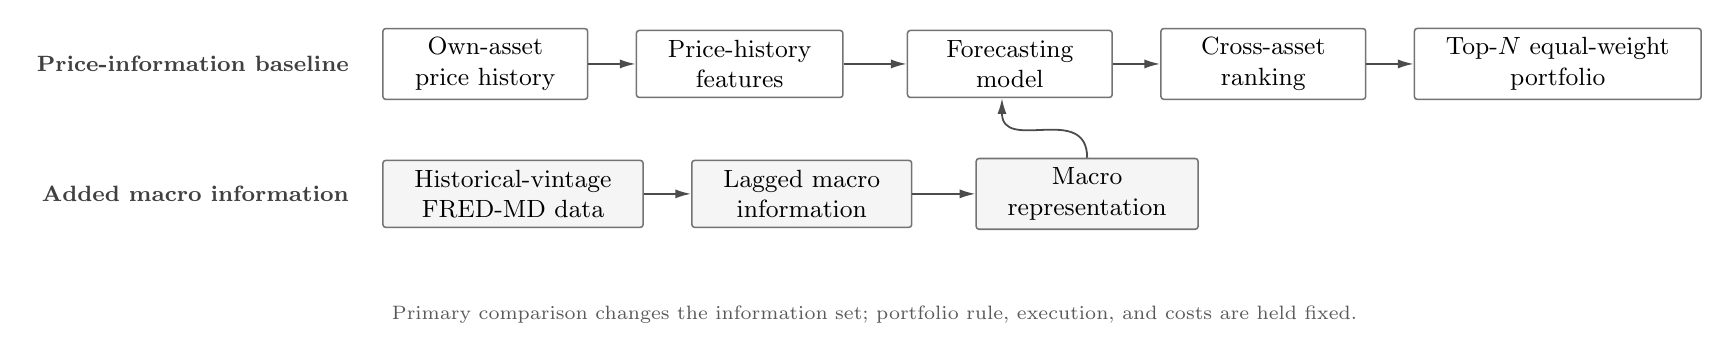
\begin{tikzpicture}[
  font=\rmfamily\small,
  box/.style={draw=black!55, rounded corners=1pt, line width=0.55pt, align=center,
              minimum height=8.5mm, inner xsep=4mm, fill=white},
  macro/.style={box, fill=black!4},
  arrow/.style={-{Latex[length=2.0mm,width=1.15mm]}, line width=0.65pt, draw=black!70},
  label/.style={font=\rmfamily\footnotesize\bfseries, text=black!75},
  note/.style={font=\rmfamily\scriptsize, text=black!65, align=center}
]

% Price-information baseline and common decision path
\node[label, anchor=east] (baseLab) at (-0.15,0) {Price-information baseline};
\node[box, right=3mm of baseLab, minimum width=26mm] (pricehist) {Own-asset\\price history};
\node[box, right=6mm of pricehist, minimum width=26mm] (pricefeat) {Price-history\\features};
\node[box, right=8mm of pricefeat, minimum width=26mm] (model) {Forecasting\\model};
\node[box, right=6mm of model, minimum width=26mm] (rank) {Cross-asset\\ranking};
\node[box, right=6mm of rank, minimum width=27mm] (portfolio) {Top-$N$ equal-weight\\portfolio};
\draw[arrow] (pricehist) -- (pricefeat);
\draw[arrow] (pricefeat) -- (model);
\draw[arrow] (model) -- (rank);
\draw[arrow] (rank) -- (portfolio);

% Added macro information enters only before the common model/ranking path
\node[label, anchor=east] (macroLab) at (-0.15,-1.65) {Added macro information};
\node[macro, right=3mm of macroLab, minimum width=26mm] (fred) {Historical-vintage\\FRED-MD data};
\node[macro, right=6mm of fred, minimum width=26mm] (lag) {Lagged macro\\information};
\node[macro, right=8mm of lag, minimum width=26mm] (repr) {Macro\\representation};
\draw[arrow] (fred) -- (lag);
\draw[arrow] (lag) -- (repr);
\draw[arrow] (repr.north) .. controls +(0,7mm) and +(0,-7mm) .. ([xshift=-1.0mm]model.south);

\node[note, anchor=west] at ([yshift=-11mm]fred.south west) {Primary comparison changes the information set; portfolio rule, execution, and costs are held fixed.};

\end{tikzpicture}
\end{document}
